\documentclass{package/notes}

%%%%%%%%%% Default Package %%%%%%%%%%%%%
\usepackage{package/color-env}
%%%%%%%%%% %%%%%%%%%%%%%%% %%%%%%%%%%%%%

%%%%%%%%%% Required Packages %%%%%%%%%%%%%
\usepackage{background}
\usepackage[object=vectorian]{pgfornament} %% used in title.tex
\usepackage{calligra} %%% (optional) to make the Title text beautiful 
%%%%%%%%%%%%%%%%%%%%%%%%

\usepackage{lipsum}  %% for dummy text 
\usepackage{amssymb,amsmath,amsfonts}  %%% for maths
%%%%%%%%%%%%%%%%%%%%%%%%%%%%%%%%%%%%%

%%%%%% Optional Packages %%%%%%%
\usepackage{lettrine} %% for nice looking 
\usepackage{GoudyIn} %% first Letter of the paragraph

\renewcommand{\LettrineFontHook}{\color{black}\GoudyInfamily{}}
% \LettrineTextFont{\itshape}
\setcounter{DefaultLines}{3}%
%%%%%%%%%%%%%%%%%%%%%%%%%%%%%%%%%%%%%
\usepackage{fourier-orns}

\backgroundsetup{contents={}}

%\usepackage{xcolor}
%\pagecolor[rgb]{0,0,0}
%\color[rgb]{0.75,0.3,0.58}
\newcommand{\R}{\mathbb{R}}
\newcommand{\Z}{\mathbb{Z}}
\renewcommand{\P}{\mathbb{P}}
\newcommand\SmallMatrix[1]{{%
  \tiny\arraycolsep=0.3\arraycolsep\ensuremath{\begin{pmatrix}#1\end{pmatrix}}}}

\begin{document}
\newpage

\begin{titlepage}

  %%%%%%%%%%%%%%%%%%%%%%%%%%%%%%%%%%%% Inspired From  %%%%%%%%%%%%%%%%%%%%%%%%%%%%%%%%%%%%%%%%%%%%%%%%% 
  %%%%  https://www.reddit.com/r/LaTeX/comments/j9d739/hello_world_in_latex_is_a_lot_cooler/   %%%%%
  %%%%%%%%%%%%%%%% If this doesn't look nice then you may remove it %%%%%%%%%%%%%%%%%%%%%%%%%%
  
  \backgroundsetup{
  scale=1,
  opacity=1,
  angle=0,
  color=black,
  contents={
  
\begin{tikzpicture}[color=black, every node/.style={inner sep= 15pt}]
  \node (NW) [anchor=north west] at (current page.north west){\pgfornament[width=2.5cm] {131}};
  \node (NE) [anchor=north east] at (current page.north east){\pgfornament[width=2.5cm, symmetry=v]{131}};
  \node (SW) [anchor=south west] at (current page.south west){\pgfornament[width=2.5cm, symmetry=h]{131}};
  \node (SE) [anchor=south east] at (current page.south east){\pgfornament[width=2.5cm, symmetry=c]{131}};
  \foreach \i in {-4,0,4}
  \node[anchor=north,xshift=\i cm] at (current page.north){\pgfornament[scale=0.25,symmetry=v]{71}};
  \foreach \i in {-4,0,4}
  \node[xshift=\i cm, yshift=32.25 pt] at (current page.south){\pgfornament[scale=0.25,symmetry=v]{71}};
  \foreach \i in {-8,-4,0,4,8}
  \node[yshift=\i cm, xshift=32.25pt, rotate=90] at (current page.west){\pgfornament[scale=0.25,symmetry=v]{71}};
  \foreach \i in {-8,-4,0,4,8}
  \node[yshift=\i cm, xshift=-32.25pt, rotate=90] at (current page.east){\pgfornament[scale=0.25,symmetry=v]{71}};
  \foreach \i in {-11,-9,...,7,9}
  \node[anchor=west, yshift=\i cm, xshift=52.25pt, rotate=90] at (current page.west){\pgfornament[scale=0.1]{80}};
  \foreach \i in {-11,-9,...,7,9}
  \node[anchor=east, yshift=\i cm, xshift=-52.25pt, rotate=-90] at (current page.east){\pgfornament[scale=0.1]{80}};
  \end{tikzpicture}
  }}
  
  %%%%%%%%%%%%%%%%%%%%%%%%%%%%%%%%%%%%%%%%%%%%%%%%%%%%%%%%%%%%%%%%%%%%%%%%%%%%%%%%%%%%%%%%%%%%%%%%%%%%%%%%%%%%%%%%%%
  
  \centering % Centre everything on the title page
      
  \scshape % Use small caps for all text on the title page
  
  \vspace*{\baselineskip} % White space at the top of the page
  
  %------------------------------------------------
  %	Title
  %------------------------------------------------
  
  \rule{\textwidth}{1.6pt}\vspace*{-\baselineskip}\vspace*{2pt} % Thick horizontal rule
  \rule{\textwidth}{0.4pt} % Thin horizontal rule
  
  \vspace{0.75\baselineskip} % Whitespace above the title
  
  {\huge \calligra{ Applied Linear Algebra }\\} % Title
  
  \vspace{0.75\baselineskip} % Whitespace below the title
  
  \rule{\textwidth}{0.4pt}\vspace*{-\baselineskip}\vspace{3.2pt} % Thin horizontal rule
  \rule{\textwidth}{1.6pt} % Thick horizontal rule
  
  \vspace{2\baselineskip} % Whitespace after the title block
  
  %------------------------------------------------
  %	Subtitle
  %------------------------------------------------
  
  \LARGE{MATH363} 
  
  \vspace*{3\baselineskip} % Whitespace under the subtitle
  
  
  
  \vspace{0.5\baselineskip} 
  
  {\scshape   \LARGE Dr. McKenzie\\ } % Editor list
  
  \vspace{0.2\baselineskip} 
  
  \textit{\Large Gonzaga University} 
  
  \vfill 
  
  %------------------------------------------------
  % Author
  %------------------------------------------------
  
  \begin{figure}[!h]
      \centering
      
\includegraphics[width = 4cm, height= 3cm]{resource/images/Gonzaga_University_Logo.jpg}%% include the university icon here
  \end{figure}
  \vspace{0.3\baselineskip} 
  
  
  {\large Edited by\\  Cameron Williamson}
  \end{titlepage}
\tableofcontents

\chapter{Linear Algebraic Systems}
\newpage
\section{First-Order Differential Equations}

In this chapter, methods will be given for solving first- order differential equations. First-order means that the first derivative of the unknown function is the highest derivative appearing in the equation. This implied that the most general first-order differential equation has the form $F(t,x,t')=0$ for some function $F$, in this chapter, we will assume that the equation can be solved explicitly for $x'$. This means that our first-order differential equations can always be put in the form:

\[
  x'=f(t,x)
\]

where $f$ denotes an arbitrary function of two variables. To see why such an assumption makes sense, supposed the differential equation is:

\[
  (x'(x))^2+4x'(t)+3x(t)=t.
\]

It would be messy, but not impossible to use the quadratic formula to extract two differential equations of the form $x'=f(t,x)$ from this quadratic equation. However, one could also imagine equations where solving for $x'(t)$ is not even possible, and in such a case, some of our methods might not be applicable.

The material in this chapter will cover several analytic methods for solving first-order differential equations, each requiring the function $f$ to have a special form. Two different graphical methods are also described; one for the general equation depending only on $x$. Numerical methods for first-order equations are introduced and theoretical issues of existence and uniqueness of solutions are discussed.

\subsection{Separable First-Order Equations}

  The first analytic method we will consider applies to first-order equations that can be written in the form

  \[
    \frac{dx}{dt} = g(t)h(t);
  \]

  that is, when the function $f(t, x)$ can be factored into a product of a function of $t$ times a function of $x$. Such a differential equation is called separable. 

  \begin{problem}
    Determine which of the following first-order differential equations are separable. Hint: try to factor the right- hand side if the equation does not initially appear to be separable.

    \[
      x' = xt + 2x\to x' = x(t + 2)\to g(t) = t + 2,h(x) = x\\
    \]

    \[
      x' = x + \cos (t)\\
    \]
    
    \[
      x' = xt^2 + t^2 - tx\to x' =(t^2 - t)(x + 1)\to g(t) =(t^2 - t),h(x) =(x + 1)\\
    \]

    \[
      x' = x^2 + x + 3\to x' = (1)(x^2 + x + 3)\to g(t) = 1,h(x) = x^2 + x + 3
    \]

    \begin{enumerate}
      \item 
        If $h(x) = 1,$ the separable equation $x'=g(t)$ is just an integrating problem and the solution is 
        \[
          x=\int g(t)dt;
        \]
        that is, $x$ is just the **indefinite integral** of the function $g(t)$. Remember that this means that $x$ can be *any* function $G(t)$ such that $G'(t)=g(t)$, and this introduces an arbitrary constant into the solution. As an example, the solution of $x'=t+1$ is 

        \[
          x(t)=\int(t+1)dt=\frac{t^2}{2}+t+ c
        \]

        Even in this simple case the solution is an infinite one-parameter family of functions.
      
      \item If $g(t)=1$, the separable equation $x'=h(x)$ is called an **autonomous** first-order differential equation. Unless $h(x)$ is a constant, it is no longer possible to solve the equation by simple integration, and the method given below must be used. Autonomous first-order differential equations are important and will be investigated more thoroughly in section 2.7. In the above examples, only the last equation is autonomous. The other three contain functions of $t$ (other than the unknown function $x(t)$) on the right-and side.
    \end{enumerate}
  \end{problem}

  \begin{problem}
    Solve the differential Equation $\frac{dx}{dt}=-tx^2$.

    Solution. Split $dx/dt$ into two pieces, $dx$ and $dt$, and do a bit of algebra to write:

    \[
      - \frac{dx}{x^2} = tdt
    \]

    Integrate each side with respect to its own variable to obtain:

    \[
      \int \left( - \frac{1}{x^2}\right) =\int tdt\to \frac{1}{x} = \frac{t^2}{x} + C.
    \]

    where the arbitrary constants on each side have been collected on the right. Solve this equation for x to obtain the one parameter family of solutions

    \[
      x=\frac{1}{(t^2/2)+C}.
    \]

    We should check that the function $x(t)$ does satisfy the differential equation for any value of the constant C. It appears that this method works, but splitting $dx/dt$ into two pieces is not a mathematically condoned operation; therefore, a justification of the method needs to be given.

    If an equation is separable, and $x'(t)$ is written as $dx/dt$, both sides of the equation $dx/dt=g(t)h(x)$ can be divided by $h(x)$, and the equation becomes

    \[
      \frac{1}{h(x(t))}\left(\frac{dx}{dt}\right)dt=\int g(t)dt+C.
    \]

    The method of simple substitution can be applied to the integral on the left. If we substitute $u=x(t)$, then $du=(dx/dt)dt$, and the equation becomes

    \[
      \int\frac{1}{h(u)}du=\int g(t)dt+C.
    \]

    Now let $H(u)$ be any function such that $H'(u)=1/h(u)$ and $G(t)$ any function with $G'9t)=g(t)$. Then the equation above implies that

    \[
      H(u)+C_1=G(t)+C_2\to H(u)=G(t)+C,
    \]

    Where C is the constant $C_2-C_1$

    Replacing $u$ again by $x(t)$:

    \[
      H(x(t))=G(t)+ C
    \]
  \end{problem}

  Check carefully that the expression $H(x)=G(t)+C$ is exactly the same as the solution obtained above. It is an **implicit solution** of $-dx/x^2=tdt$; that is, it defines a relationship between the unknown function $x$ and its independent variable $t$. If it can be solved explicitly for $x$ as a function of $t$, the result is called an **explicit solution of the differential equation. As expected, the integration produces an infinite on-parameter family of solutions

  \begin{theorem}
    TTo solve a separable first-order differential equation, $x'(t)=g(t)h(x)$:
    \begin{itemize}
      \item Write the equation in the form $dx/dt=g(t)h(x)$.
      \item Multiply both sides by $dt$, divide by $h(x)$, and integrate, to put the equation in the form 
        \[
          \int \frac{1}{h(x)}dx =\int g(t)dt.
        \]
      \item Find any function $H(x)$ such that $H'(x)=1/h(x)$ and any function $G(t)$ such that %G'(t)=g(t).
      \item Write the solution as $H(x)=G(t)+C$
      \item If possible, solve the equation from the previous step explicitly for x, as a function of t.
    \end{itemize}
  \end{theorem}

\subsection{Solving Linear ODEs}

 \begin{definition}
   An ODE is linear for the dependent variable $y$ if it is homogeneous when $g(x)=0$ and otherwise it is non-homogeneous.
   \[
     a_1(x)\frac{dy}{dx}+a_0(x)y=g(x)
   .\] 
   The standard form of a linear ODE is
   \[
     \frac{dy}{dx}+P(x)y=f(x)
   .\] 
 \end{definition}
 
 If the homogeneous ODE is separable: $y=e^{-\int P(x)dx}$, and $y_c=cy_1(x)$ where $y_1=e^{-\int P(x)dx}$. For a non-homogeneous ODE, we need to use the process of “variation of parameters”. First we need to find the function $u$ so that $y_p=u(x)y_1(x)=u(x)e^{-\int P(x)dx}$, and then we follow the following steps

 \begin{enumerate}
   \item Put in standard form
   \item Determine $P(x)$ and integrating factor $e^{\int P(x)dx}$.
   \item Multiply std form by integrating factor.
   \item Write \[
       \frac{d}{dx}\left[e^{\int P(x)dx}y\right]=e^{\int P(x)dx}f(x)
   .\] 
  \item Integrate both sides.
 \end{enumerate}

\subsection{}

\subsection{Existence and Uniqueness of Initial Value Problems}

  Given an initial value problem, how can I know that a solution exists, and if so, the uniqueness of that solution.

  \begin{problem}
    $\frac{dx}{dt}=\sqrt{x}$, $x(0)=0$ has two solutions. These solutions are $x(t)=\frac{t^2}{4}$ and $0$. We can change the initial condition to be $x(0)=5$. We can separate our values to get:

    \[
      x(t) =\left(\frac{t}{2} + \sqrt{5}\right)^2
    \]
    
    If we change the initial condition to $x(5)=-5$ we get no solutions. We can also change the initial condition to $x(5)=0$ which gives us two solutions:

    \begin{align*}
      x(t) =\left(\frac{t - 5}{2}\right)^2\\
      x(t) = 0
    \end{align*}
  \end{problem}

\subsection{Exact Ordinary Differential Equations}

  This highlights an analytic technique to find the solutions to an ordinary differential equation. This technique depends on if we are able to write an ODE in the form $\frac{d}{dx}(F(x,y(x)))=0$. How can we tell if this is possible? 

    We can determine this by using the multi-variable chain rule from calculus 3:

    \[
      \frac{d}{dx}(F(x,y(x))) = \frac{\partial F}{\partial x} + \frac{\partial F}{\partial y} \frac{dy}{dx} = 0 
    \]

    Now in order to actually solve the ordinary differential equation, we will turn the equation above into something that we can work with:

    \[
      M(x,y) + N(x,y)\frac{dy}{dx} = 0
    \]

    Now we ask, does $f(x,y)$ exist such that $\frac{\partial F}{\partial x} =  M(x,y)$ and $\frac{\partial F}{\partial y} = N(x,y)$? We can test this by checking to see if we can do the following:

    \[
      \frac{\partial^2F}{\partial x\partial y}=\frac{\partial^2 F}{\partial y\partial x}\rightarrow\boxed{\frac{\partial M}{\partial y}=\frac{\partial N}{\partial x}}
    \]

    If it passed the test, we use the equations to find $F(x,y)$, and then we can use $F(x,y(x))=C$ to find the solution to the problem.

    \begin{problem}
      Calculus 3 example. Consider a field $\vec{v}=<2y+4x,2x-5y>$. Is this a gradient field? If so, what is its potential function. In order to find this, there must be a function $f(x,y)$ such that $\bigtriangledown f=\vec{v}$.
    
    
      \[
        {\partial f}{\partial y}\big>=<6xy,2x-5y>\\
      \]
  
      \begin{align*}
        \frac{\partial f}{\partial x}=6xy,&& \frac{\partial f}{\partial y}=2x-5y
      \end{align*}
  
      Therefore, we know that $f_{xy}=f_{yx}$ Now we just need to set the two equations equal to each other and solve:
  
      \[
        \frac{\partial}{\partial y}(2y+4x)\stackrel{?}{=}\frac{\partial}{\partial x}(2x-5y)
      \]
  
      And we can solve that equation algebraically and get $2=2$, therefore this is the solution to the ordinary differential equation
  
    \end{problem}

    \begin{problem}
      Solve $(4x+2y)+(2x-5y)\frac{dy}{dx}=0$. We should set $M(x,y)=4x+2y$ and set $N(x,y)=(2x-5y)$.

    \begin{enumerate}
      \item Testing to see if $\frac{\partial M}{\partial y}=\frac{\partial N}{\partial x}$
        \[
          \frac{\partial}{\partial y}(4x+2y)\stackrel{?}{=}\frac{\partial}{\partial x}(2x-5y)
        \]
      \item Now we need to find $F(x,y)$:
        \begin{align*}
          \frac{\partial F}{\partial x}=4x+2y && \frac{\partial F}{\partial y}=2x-5y\\
          F(x,y)=\int(4x+2y)dx=2x^2+2xy+c_y, && F(x,y)=\int(2x-5y)dy=2xy-\frac{5}{2}y^2+c_x
        \end{align*}
        We can determine that $c_y=\frac{5}{2}y^2$ and $c_x=2x^2$ by looking at the two equations next to each other. Therefore, we know that $F(x,y)=2x^2+2xy-\frac{5}{2}y^2$.
    \end{enumerate}
    Our resulting solution is:

    \[
      \boxed{2xy-\frac{5}{2}y^2+2x^2=C}
    \]

    This was an implicitly defined solution, so $F(x,y)=2xy-\frac{5}{2}y^2+2x$, and our ode is:
    
    \begin{align*}
      \frac{d}{dx}\left[2xy(y)-\frac{5}{2}(y(x))^2+2x^2\right]=\frac{d}{dx}[C]\\
      (2y+2xy')-\frac{5}{2}2(y)+4x=0\\
    \end{align*}

    \paragraph{Example 2} Solve the differential equation,
    
    \[
      2x^2y+e^y+(x^3+xe^y-2y)\frac{dy}{dx}=0. 
    \]

    We can see that $3x^2y+e^y = M(x,y)$ and $(x^3+xe^y-2y)\frac{dy}{dx}=0$.

    We can test this by checking to see if:
    
    \[
      \frac{\partial M}{\partial y}\stackrel{?}{=}\frac{\partial N}{\partial x}
    \]

    and by taking the partial derivatives of each of the equations, we can see that $3x^2+e^y=3x^2+e^y$. Now that we know that this is an exact ordinary differential equation, we need to solve for $F(x,y)$. In order to find $F(x,y)$, we must do 

    \begin{align*}
      \frac{\partial F}{\partial x}=M && \frac{\partial F}{\partial y}=N.
      \end{align*}

      This means that 

      \begin{align*}
        F(x,y)=\int(3x^2y+e^y)dx && F(x,y)=\int(x^3+xe^y-2y)dy\\
        =x^3y+xe^y+C_y && =x^3y+xe^y-y^2+C_x\\
      \end{align*}

      So, $F(x,y)=x^3yxe^y-y^2$, and our solution is:

      \[
        \boxed{x^3y+xe^y-y^2=C}\\
      \]

      Now we need to find a solution that satisfies the initial value problem, $y(-2)=1$.
      
      \begin{align*}
        (-2)^3(1)+(-2)e^1-(1)^2&=C\\
        -8-2e-1&=C\\
        -9-2e&=C\\
      \end{align*}

      Which results in our particular solution being:

      \[
        \boxed{x^3y+xe^y-y^2=-9-2e}
      \]
    \end{problem}

  \subsubsection{Substitution}
    Sometimes we can make a substitution that turns one ordinary differential equation into one that we can solve.
    
    \begin{problem}
      Let's take the equation $\frac{dy}{dx}=\frac{1-x-y}{x+y}$. In order to do this you need to trade out $y(x)$ for $u(x)$:

      \[
        \frac{dy}{dx}=\frac{du}{dx}-1
      \]

      \[
        \frac{du}{dx}-1=\frac{1-u}{u}=\frac{1}{u}-1
      \]

      After we do those steps, we can see that this is a separable ordinary differential equation, and we can use the normal method to solve a separable equation:

      \[
        \begin{aligned}
          \int udu&=\int1dx\\
          \frac{u^2}{2}&=x+C\\
          u^2&=2x+D\leftarrow D=2C\\
          (x+y)^2&=2x+D\rightarrow x+y=\pm\sqrt{2x+D}\\
          y&=-x\pm\sqrt{2x+D}
        \end{aligned}
      \]

      Where the initial condition determines the last equation above. Now we need to solve for the initial condition of $y(6)=4$, and we can do this by just plugging in the values, and determining the sign on the square root:

      \[
        \begin{aligned}
           4&-6\pm\sqrt{12+D}\\
          10&=\pm\sqrt{12+D}\\
          D&=88\to y(x)=-x+\sqrt{2x+88}\\
        \end{aligned}
      \]
    \end{problem}

  \subsubsection{Bernoulli Ordinary Differential Equations}

    We use Bernoulli's solution to an ordinary differential equation if the equation can be written in the form $\frac{dx}{dt}+p(t)x=q(t)x^n$, where if $n=0$, the equation is linear and where if $n=1$, the equation is both linear and separable. We can do a substitution for Bernoulli ordinary differential equations where we let $v=x^{1-n}$, and we trade out $x(t)\to v(t)$ to turn the differential into a linear differential. Another formula we can use for plugging in to find the separable ordinary differential equation is $\frac{du}{dx}+(1-n)p(x)u=(1-n)q(x)$, but we do not have an example to show for that method. 

    \begin{problem}
      Consider the Ordinary differential equation $t\frac{dy}{dt}+y=\frac{1}{y^2}$, and solve. Our first step for this problem is to divide both sides by $t$ to rearrange it into the Bernoulli form:

      \[
        \frac{dy}{dt}+\frac{1}{t}y=\frac{1}{t}y^-2
      \]

      Because $y$ is our dependent variable, we will be looking for our $n$ value, and we will find it on the $y$ on the right-hand side. This gives us $n=-2$. Now we need to let $v(t)=y^{1-(-2)}=y^3$ and this means that $y(t)=(v(t))^{1/3}$. Now wee need to take the differential of this equation in order to find a substitution for $\frac{dy}{dt}$:

      \begin{align*}
        \frac{dy}{dt}=\frac{1}{3y^2}\frac{dv}{dt}\\
        \frac{dv}{dt}=3y^{-2}\frac{dy}{dt}\\
      \end{align*}

      Once we have found a substitution for $\frac{dy}{dt}$, we can simply plug in our equation and solve for $v(t)$:

      \[
        \frac{1}{3y^2}\frac{dv}{dt}+y=\frac{1}{y^2}
      \]

      \[
        \frac{t}{3}\frac{dv}{dt}+y^3=1
      \]

      We solve for $v(t)$, and then we can use the integrating factors method to solve the ordinary differential equation:

      \[
        \begin{aligned}
          \frac{dv}{dt}+\frac{3}{t}v&=\frac{3}{t}\\
          \mu(t)&=e^{\int\frac{3}{t}dt}=e^{3ln(t)}=t^3\\
          t^3\frac{dv}{dt}+3t^2v&=3t^2\\
          \frac{d}{dt}(t^3v)&=3t^2\\
          \int t^3v&=\int3t^2dt=t^3+C\\
          v(t)&=1+\frac{C}{t^3}\to y(t)=(v(t))^{\frac{1}{3}}\\
        \end{aligned} 
      \]\\

      Now we just need to let $v(t)=y^3$ and plug this back into the equation to get $y(t)=\left(1+\frac{C}{t^3}\right)^{\frac{1}{3}}$ as our final solution.
    \end{problem}

    Homogeneous ordinary differential equations can be written in the form $\frac{dx}{dt}=f\left(\frac{x}{t}\right)$. This means that if we just substitute $v$ for $\frac{x}{t}$, we will turn the Homogeneous equation into a separable ordinary differential equation.

    \begin{problem}
      Consider the homogeneous ODE, $(5y-2x)\frac{dy}{dx}=4x+2y$. We can divide the $5y-2x$, so we will end up with the equation

      \[
        \frac{dy}{dx}=\frac{4x+2y}{5y-2x}=\frac{4+\frac{2y}{x}}{5\frac{y}{x}-2}
      \]

      The reason we can make this change is that we are dividing everything on the left side by $x$ to get it in the form $\frac{y}{x}$. Our next step is to trade out $y(x)$ for $v(x)$:

      \[
        \frac{4+2v}{5v+2}=v+x\frac{dv}{dx}\\
      \]

      Which we can further simplify into $\frac{dv}{dx}=\frac{1}{x}\left(\frac{4+2v}{5v-2}-v\right)$. Now, we are able to solve this as a separable ordinary differential equation:

      \[
        \begin{aligned}
          \frac{dv}{dx}&=\frac{1}{x}\left(\frac{4+4v-5v^2}{5v-2}\right)\\
          \frac{5v-2}{4+4v-5v^2}dv&=\frac{1}{x}dx\\
        \end{aligned}
      \]

      Now we need to let $u-4+4v-5v^2$, and let $du=(4-10v)dv=-2(5v-2)dv$. And then we integrate with respect to $u$ to end up with 

      \[
        \begin{aligned}
          -\frac{1}{2}\int\frac{1}{u}du&=\int\frac{1}{x}dx\\
          -\frac{1}{2}ln|u|&=ln|x|+C\\
          ln|4+4v-5v^2|&=-2ln|x|+D\\
          4+4v+5v^2&=e^{ln|x|^-2+D}\\
          &=e^{ln|x|^{-2}}e^D\\
          4+4\left(\frac{y}{x}\right)-5\left(\frac{y}{x}^2\right)&=e^{ln|x|^{-2}}A
        \end{aligned}
      \]

      \[
        \boxed{4x^2+4xy-5y^2=A}
      \]
    \end{problem}

\subsection{}
\subsection{Phase Lines and Equilibrium Solutions}

  This is a qualitative technique for autonomous ordinary differential equations. This is used for finding the long term behavior of solutions for various initial conditions. An equilibrium solution is a constant function satisfying the ODE:

  \[
    y(t)=k\to\frac{dy}{dt}=0
  \]

  and we need to look for the roots of $f(y)$.

  \begin{problem}
    Consider the ODE: $\frac{dy}{dx}=4-y^2$, we know that the equilibrium solutions (stationary points / fixed points / critical points) are $0=4-y^2$ and $y=\pm2$.  If we were to plot this as a slope field, we would see an image like the following:
  
    \begin{center}
      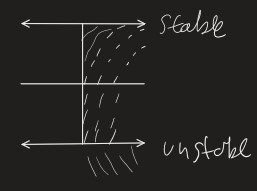
\includegraphics{resource/images/2.7 Example 1.jpg}
    \end{center}

    We need to classify each of the lines here as stable (a sink), unstable (a source), or semi-stable (a node). From this slope diagram we can make a phase diagram.

      

    The arrows in this diagram indicate whether $\frac{dy}{dx}$ is above or below $0$. We can see that the long term behavior of the solution:

    \[
      \begin{aligned}
        y_0 = y(t_0) > 2,\to y(t)\to 2\\
        - 2 < 2_0,\to y(t)\to 2\\
        y_0 <- 2, y(t)\to -\infty\\
      \end{aligned}
    \]
  \end{problem}

  Let's take a look at another example problem:

  \begin{problem}
    Compare the pivots of the two ordinary differential equations, $\frac{dy}{dt}=y^2(1-y)^2$, and $\frac{dy}{dx}=y^2(1-y^2)$.

    \begin{align*}
      \frac{dy}{dt}=y^2(1-y)^2 && \frac{dy}{dt}=y^2(1-y^2)\\
      0=y^2(1-y)^2 && 0=y^2(1-y^2)\\
      && y=0,\pm1\\
    \end{align*}
    From finding the equilibrium points of the differential equations, we can now craft a pivot diagram:\newline
    \begin{center}
    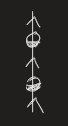
\includegraphics{resource/images/2.7 Example 2-1.jpg}
    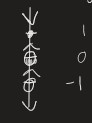
\includegraphics{resource/images/2.7 Example 2-2.jpg}
    \end{center}

    From this we can see that in the long term, the equations are going to look like this:

    \begin{align*}
      y_0<0,y(t)\to0\\
      0<y_0<1,y(t)\to1\\
      1<y_0,y(t)\to\infty\\
    \end{align*}
  \end{problem}

  \subsubsection{Bifurcations}

  For ordinary differential equations with a parameter, there are times that a small change in the value of the parameter results in a huge change in the behavior of the solutions. It causes a change in the number or stability of the equilibrium solutions.

  \begin{problem}
    Find the bifurcation value for 

    \[
      \frac{dp}{dt}=0.5p\left(1-\frac{p}{100}\right)-H
    \]

    The first step for finding a bifurcation for an equation is finding the equilibrium solutions. In order to do that, we set equation (2.69) equal to 0 and then rearrange it, so it is in the form

    \[
      p^2-100p+250H=0
    \]

    In this case, we are going to need to use the quadratic formula to find the equilibrium points:

    \begin{align*}
      p=\frac{100\pm\sqrt{10000-1000H}}{2}\\
      =50\pm5\sqrt{100-10H}
    \end{align*}
    We can determine that our bifurcation value is $H=10$, because if we take what's under the square root, and set it equal to zero we can find those values.
    Now we can plot our bifurcations:
    \begin{center}
      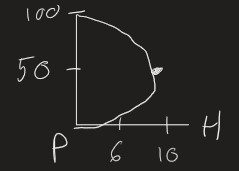
\includegraphics{resource/images/2.7 Example 3 1.jpg}
    \end{center}
  \end{problem}
  \section{Numerical Methods\footnote{We got here from 4.1}}

\chapter{Inner Products and Norms}

\section{Inner Products}

\section{Inequalities}

\section{Norms}

\section{Positive Definite Matrices}

\section{Completing the Square}

\section{Complex Vector Spaces}
\newpage
\section{Systems of Ordinary Differential Equations}
\subsection{}
Systems of ordinary differential equations have 1 dependent variable and 1 independent variable. Let's look at an example.

\begin{eg}
  Here is a system of 3 first order ordinary differential equations of dimension 3 
  \begin{align*}
    x'&=4x-7y+z^2\\
    y'&=2t-e^{t}y-z\\
    z'&=z^2+y^2-yx
  .\end{align*}
\end{eg}

We can also turn higher order ODE's into systems of first-order ODEs.
\begin{eg}
  Consider the equation $x''+7x''+7tx'+6x=t^2$. If we let $y=x',z=x''=y',x'''=z'$, then using the ODE,
  \[
  z'=t^2-6x+7ty-7z
  ,\]
  we can make a system of nonlinear, nonautonomous, nonhomogeneous ordinary differential equations.\footnote{After this system we went to chapter 2.6}
  \begin{align*}
    x'&=y\\
    y'&=z\\
    z'&=t^2-6x+ty-7z
  .\end{align*}
\subsection{Matrix Algebra}
A matrix is a rectangular array of numbers. 
\begin{eg}
  Consider $A=\begin{pmatrix} 2&3&1\\4&5&0 \end{pmatrix} $. $A$ has 2 rows and 3 columns, so its size is $2\times 3$. The $a_{ij}$ is an entry in $A$'s $i^{th}$ row and $j^{th}$ column.
\end{eg}
\begin{eg}
  Consider $B=\begin{pmatrix} 5&0&0\\0&-1&0\\0&0&3 \end{pmatrix} $, which is a $3\times 3$ matrix. This is also a square matrix, due to the size. $B$ is also a diagonal matrix, because it's only nonzero entries are on the main diagonals.
\end{eg}
An upper triangular matrix looks like 
\[
  \begin{pmatrix} 5&2&0\\0&-1&3\\0&0&3 \end{pmatrix} 
.\] 
A lower triangular matrix looks like
\[
  \begin{pmatrix} 5&0&0\\ \pi&-1&0\\-1&-\frac{1}{2}&3 \end{pmatrix} 
.\] 
\end{eg}
We can add and subtract matrices element-wise, but only if the matrices have the same size. We can also multiply a matrix by a scalar
\[
  3\begin{pmatrix} 4&5\\6&7 \end{pmatrix} =\begin{pmatrix} 12&15\\18&21 \end{pmatrix} 
.\] 
A row vector is $\begin{pmatrix} 2&3&1 \end{pmatrix} $, in this case the size would be $1\times 3$. A column vector looks like $\begin{pmatrix} 2\\3\\1 \end{pmatrix} $ with the size $3\times 1$. The zero vector is of size $n\times n$, and has $0$ in every index in the matrix. The transpose of a matrix reverses all of the columns and rows. Consider
\[
  \begin{pmatrix} 2&3&1\\4&5&6 \end{pmatrix} ^{T}=\begin{pmatrix} 2&4\\3&5\\1&6 \end{pmatrix} 
.\] 
Here are the properties of a transpose:
\begin{itemize}
  \item $\left( A^{T} \right)^{T}=A $
  \item $\left( A+B \right) ^{T}=A^{T}+B^{T}$
  \item $(kA)^{T}=kA^{T}$
  \item $\left( AB \right) ^{T}=B^{T}A^{T}$
\end{itemize}
Now we are going to start talking about matrix multiplication. Matrix multiplication is like the dot product. The $(i,j)^{th}$ entry of $AB$ is the dot product of the $i^{th}$ row of $A$ w/ $j^{th}$ column of $B$. Consider the following
\[
  \begin{pmatrix} 1&2&3 \end{pmatrix} \begin{pmatrix} 4\\5\\6 \end{pmatrix} =(1\times 4)+(2\times 5)+(3\times 6)= 32
.\] 
In order to do matrix multiplication, rows of $A$ must match the columns of $B$ and vice versa. Matrix multiplication is not commutative. 
\begin{eg}
  If we let $A=\begin{pmatrix} 1&4\\5&10\\8&12 \end{pmatrix}$ and $B=\begin{pmatrix} -4&7&-3\\1&-3&2 \end{pmatrix} $. Does $AB=BA$? This is not true, because matrices are equal if and only if all entries are equal. If we just multiply $BA$, we get \[
  \begin{pmatrix} -4&7&-3\\1&-3&2 \end{pmatrix}\begin{pmatrix} 1&4\\5&10\\7&12 \end{pmatrix}  = \begin{pmatrix}2&8\\2&-2\end{pmatrix} 
  .\] 
\end{eg}
Here are some properties of matrices. 
\begin{note}
  We must maintain the order from left to right.
\end{note}
\begin{itemize}
  \item $A(B+C)=AB+BC$
  \item $(A+B)C=AC+BC$
  \item $k(AB)=(kA)B=A(kB)$
  \item $ABC=(AB)C=A(BC)$
\end{itemize}
The identity matrix is a square diagonal matrix with ones on the diagonal. For example, the identity matrix of dimension 3 and 4 are the following 
\begin{align*}
  I_3&=\begin{pmatrix} 1&0&0\\0&1&0\\0&0&1 \end{pmatrix} \\
  I_4&=\begin{pmatrix} 1&0&0&0\\0&1&0&0\\0&0&1&0\\0&0&0&1 \end{pmatrix} 
.\end{align*}
With the identity matrix, if we multiply any matrix by the identity matrix, then we get the same answer. Back in lesson 2, we were given the general solution to a Cauchy-Euler ordinary differential equation as \[
  x(t)=C_1(1)+C_2t^3+C_3 \frac{1}{t^2}
.\] Let's find a particular solution satisfying $x(1)=2,x'(1)=4,x'(1)=0$. We can do this by taking the derivative and second derivative of our functions to get 
\begin{align*}
  x'(t)=3C_2t^2-2C_3t ^{-3}\\
  x''(t)=6C_2t+6C_3t ^{-4}
.\end{align*}
Now using our initial conditions
\begin{align*}
  x(1)=C_1+C_2+C_3=2\\
  x'(1)=3C_2-2C_3=4\\
  x''(1)=6C_2+6C_3=0
.\end{align*}
We can rewrite this in matrix form as \[
  \begin{pmatrix} 1&1&1\\0&3&-2\\0&6&6 \end{pmatrix} \begin{pmatrix} C_1\\C_2\\C_3 \end{pmatrix} =\begin{pmatrix} 2\\4\\0 \end{pmatrix} 
.\] We will call the first matrix, $A$, the second matrix, $\vec{x}$, and the third matrix, $\vec{b}$, so we must solve $A\vec{x}=\vec{b}$ for $\vec{x}$. We can solve this by doing the following techniques
\begin{enumerate}
  \item Cramer's Rule (See book appendix)
  \item Gaussian elimination
  \item (Left)-multiply by $A^{-1}$
  \item MATLAB: rref or $A / B$
\end{enumerate}

\begin{theorem}
  This is the invertible matrix theorem. If $A$ is square, either all of case 1 or all of case 2 statements are true. Either $A$ is non-singular [good] or $A$ is singular [bad]. \newline Considering case 1
  \begin{itemize}
    \item $det(A)\neq 0$
    \item $A\vec{x}=\vec{b}$ has exactly one solution $\vec{x}$ for each $\vec{b}$.
    \item $A\vec{x}=\vec{0}$ has only the trivial solution, $\vec{x}=\vec{0}$.
    \item The rows (and columns) are linearly independent.
    \item $A^{-1}$ exists.
  \end{itemize}
  Considering Case 2
  \begin{itemize}
    \item $det(A)=0$
    \item $A\vec{x}=\vec{b}$ has zero or infinite solutions
    \item $A\vec{x}=\vec{0}$ has infinite solutions.
    \item The rows (and columns) are linearly dependent.
    \item $A^{-1}$ does not exist.
  \end{itemize}
\end{theorem}
$A^{-1}$ is a square matrix such that \[
A^{-1}A=A A^{-1}=I
.\] We find $A^{-1}$ through the following methods
\begin{enumerate}
  \item $rref(A|I)\to(I|A^{-1})$
  \item $A^{-1}=\frac{1}{det(A)}\cdot adj(A)$ where $adj(A)$ is the transpose of the cofactor matrix.
\end{enumerate}
How do we use $A^{-1}$? Given $A\vec{x}=\vec{b}$, we must solve for $x$. In order to do this, we left multiply by $A^{-1}$ to get 
\begin{align*}
  A^{-1}A\vec{x}&=A^{-1}\vec{b}\\
  I\vec{x}&=A^{-1}\vec{b}\\
  \vec{x}=A^{-1}\vec{b}
.\end{align*}
If given a general $2\times 2$ matrix, $A=\begin{pmatrix} a&b\\c&d \end{pmatrix} $, we can find the inverse by doing 
\begin{align*}
  A^{-1}&=\frac{1}{ad-bc}\begin{pmatrix} d&-c\\-b&a \end{pmatrix} ^{T}\\
        &=\frac{1}{ad-bc}\begin{pmatrix} d&-b\\-c&a \end{pmatrix} 
.\end{align*}
The trace of $A$ ($trace(A)$) is the sum along the diagonal.

\newpage
\section{Qualitative Techniques for Autonomous Systems (2D)}
This is a generalization of phase lines. Phase planes are a parametric plot of $y(t)$ vs. $x(t)$. Phase planes come up a lot in physics. Our spring mass equation \[
mx''+bx'+kx=c
,\] can be turned into a system if we let $y=x'$

\chapter{Equilibrium}
\section{Linearity}

\section{Eigenvalues and Singular Values}
\subsection{}
\subsection{Eigen Values and Eigen Vectors}

\begin{definition}
  Let $A$ be an $n\times n$ matrix. A scalar $\lambda$ is an eigenvalue of $A$ if 
  \[
  A\vec{v}=\lambda\vec{v}
  .\] 
  for some non-zero vector $\vec{v}\cdot\vec{v}$ is called the eigenvector corresponding to lambda.
\end{definition}
So\ldots
\begin{align*}
  A\vec{v}&=\lambda\vec{v}\\
  A\vec{v}-\lambda\vec{v}&=0\\
  (A-\lambda I)\vec{v}&=\vec{0}\\
.\end{align*}

Solve for $\lambda$ and $\vec{v}$. We want $\vec{v}\neq \vec{0}$. We must have 
\[
  det(A-\lambda I)=0
.\] 

\chapter{Iteration}
\chapter{Dynamics}
\pagebreak

\medskip

\printbibliography[heading=bibintoc,title={\centering Bibliography}]

\end{document}
